\section{Application} % (fold)
\label{sec:application}

In this section, we first provide an informal description of the application. Then, we go ahead and formalize the goal it
pursues.

\subsection{Informal Description} % (fold)
\label{sub:informal_description}

We introduce {\tt Social News}, a social networking application that identifies headlines from a set of news. It shares
some closeness with {\tt Google News} (see~\url{http://news.google.com}), a \emph{Google~\texttrademark} application that
identifies headlines from a collection of news retrieved from different sources on the Internet. Rather than the
centralized headline identification approach known to {\tt Google News}, {\tt Social News} uses a \emph{distributed} one.

Let $\Omega=<N_\Omega,L_\Omega>$ denote a social network, where $N_\Omega$ is a set of nodes (the members of the social
network) and $L_\Omega$ denote a set of links between elements of $N_\Omega$. For example, consider that $\Omega$ is the
social network depicted in figure~\ref{fig:sn-news-init}. At the beginning of the process, some members of the social
network possess news, which they wish to turn into headlines. Such nodes are represented in green color in the figure,
whereas the other nodes are represented in blue color. Green color nodes submit their news as a whole package by sending
a message to their immediate neighbors. A node $\nu_\ell$ will send a message of the format:
$\nu_\ell^S=<\alpha_0^\ell,\ldots,\alpha_m^\ell>$, where the $\alpha_\imath^\ell$ are the news he intends to submit. When
a node $\nu_p$ receives an invitation $\nu_\ell^S$, he can do one of the following four things:

\begin{itemize} 
	\item decline the invitation, by replying \emph{``no!''};
	\item decline the invitation, but decide to forward it to other members by replying \emph{``forward!''};
	\item accept to join the group as a simple voter, by replying \emph{``voting!''}; 
	\item accept to join the group with his own news, by replying with another invitation $\nu_p^S=<\alpha_0^p,\ldots,\alpha_k^p>$. In this case $\nu_\ell$ can reject the condition and exclude $\nu_p$
from the group or accept to compete locally with $\nu_p$. 
\end{itemize}

\begin{figure} 
	\centering 
	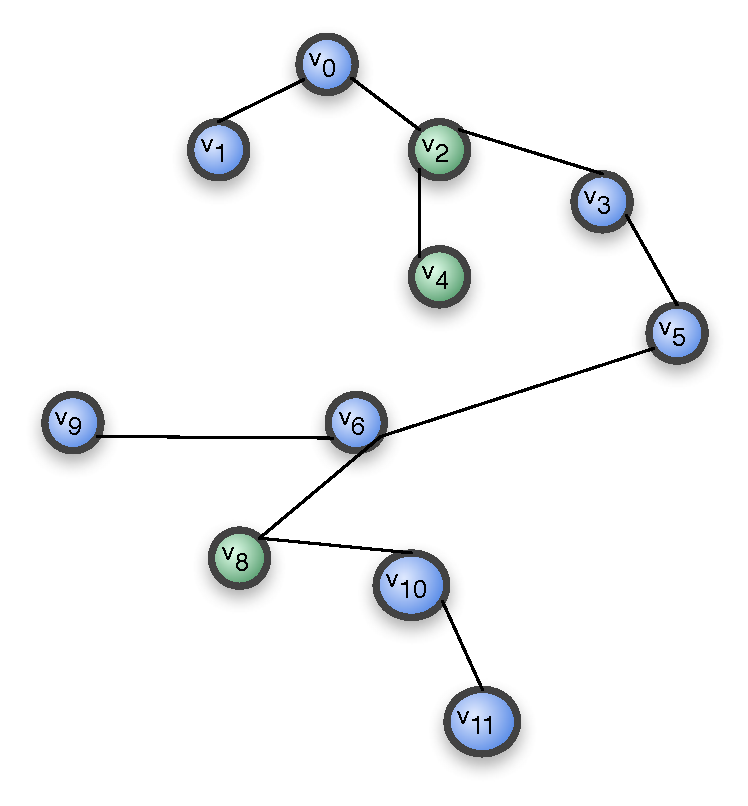
\includegraphics[width=.5\textwidth]{social_news} 
	\caption{News Social Network}
	\label{fig:sn-news-init} 
\end{figure}

In order for a node $\nu_\ell$ to change his news into headlines, he has to extend his initial group into a bigger one
so that many more network members vote for his news. This is the \emph{group extension phase}, which is constrained by
a deadline. Note that a node can join an extended group, while submitting his own news to another one. However, a node
cannot submit news to two different groups. Once an extended group is created, its members have to select their
\emph{local headlines}. These headlines will compete with those proposed by other groups. This second phase is known
as the \emph{inter-group competition} for final headline identification. Each headline identification (whether local or
global) involves a voting activity, where weights are assigned to the news on a scale of $\omega_0$ to $\omega_5$, with $\omega_0$
the lowest vote. Note that all votes remain equal, i.e., a vote cast by a \emph{popular} node and one by a \emph{totally
unknown} node are equal. Moreover, a node that submitted news to a group is neither allowed to vote for his own news, nor
can he cast ballots for other news.

While forming groups it is not allowed to form groups that are part of other groups. Forming groups requires
fine-tuned strategies. For example, nodes should decide whether they prefer small groups, where their news are likely
to be selected as local headlines, or larger groups where passing a news as a local headline becomes more competitive.
On the other hand, a large group limits competition at a global level, while smaller groups make it more difficult
at a global level. Moreover, during news transmission there is a risk of the sender node ``antagonizing'' the receiver
since all interested nodes submit their news concurrently.

% subsection informal_description (end)

\subsection{Formalization} % (fold)
\label{sub:formalization}

From the informal description above, at least two properties need to be checked in {\tt Social News}'s implementation.
These are: \begin{inparaenum}[\itshape i\upshape)] \item a node cannot submit news to more than one group; \item it is
not allowed to form groups that are part of others. \end{inparaenum} Checking these properties requires to provide formal
specifications. However, since we do not intend to discuss model checking in this paper, we simply provide the
specifications of the goals pursued in {\tt Social News}. Our specification follows a declarative approach, i.e.,
\emph{what are the nodes supposed to do, instead of how they should do it}.

Consider a social network $\Omega$ with $p$ members, $k~(k\leq p)$ of which submit news to the network and expect to turn
them into global headlines. Let $\mathcal{H}$ denote a set of headlines and $\rho_\mathcal{H}$ denote a logical formula
which is only true when as many headlines as required have been adopted.

For a node $\nu_\ell$ submitting a set of news $<\alpha_{0}^\ell,\ldots,\alpha_m^\ell>$, his goal $\rho_\ell$ is to turn at least a subset of his news set into headlines. 
\begin{equation}
	\label{eq:indgoals}
	\begin{gathered}
		\Omega\vDash\rho_\ell \iff\exists\gamma=<\alpha_\imath^\ell,\ldots,\alpha_\jmath^\ell>\subseteq\mathcal{H},
		\gamma\subseteq <\alpha_0,\ldots,\alpha_m>
	\end{gathered}
\end{equation}

The goal achieved by {\tt Social News} is to identify $N$\footnote{In this case $\rho_\mathcal{H}$ holds when the size of
$\mathcal{H}$ in $N$.} headlines from the set of news submitted to the social network. This goal is a composition of the
individual goals pursued by the nodes who submitted sets of news to the social network. Note that not all the individual
goals need to be reached before the global one is reached. We use $CTL^*$ (see~\cite{Emerson-Halpern:86}) to specify the
relationship between the global goal $\rho$ and the individual ones.

\begin{equation}
	\label{eq:appgoal}
	(F\rho_\mathcal{H}\wedge E[F\rho_0\vee F\rho_1\ldots \vee F\rho_k])\implies A[\rho]
\end{equation}

% Although straightforward, due to the expressive power of $CTL^*$, model checking this specification is out the scope of
% this paper.

% subsection formalization (end)

% section application (end)